% Ch5.tex
\chapter{Multiple-instance multiple-label learning for the classification of frog calls with acoustic event detection}
\label{cha:cha6MIML}

\textbf{Research problem}
\\
In Chapters \ref{cha:cha4EnhancedFeature} and \ref{cha:cha5WaveletFeature}, each individual recording is assumed to contain only one frog species. However, most field recordings collected by acoustic sensors have multiple frog species and a low SNR.
\\
\textbf{Research sub-question}
\\
How to classify multiple simultaneously vocalising frog species in field recordings?


\section{Overview}
\label{sec:intro}

This chapter proposes a method for the classification of multiple simultaneously vocalising frog species in field recordings. In Chapters \ref{cha:cha4EnhancedFeature} and \ref{cha:cha5WaveletFeature}, frog call classification is solved using a SISL classification framework, which cannot reflect the nature of automatically collected field recordings. Most field recordings have a low SNR and contain multiple simultaneously vocalising animals including frogs, birds, insects, and so on. This attribute makes MIML learning a natural fit for studying field recordings. Specifically, frog syllables in one audio clip (such as 10-second) are regarded as \textit{multiple instance}, and frog species included in that audio clip denotes \textit{multiple labels}. 
First, AED is used to segment frog syllables of each audio clip.
Then, acoustic features are extracted from each segmented syllable. Lastly, three MIML classifiers are used for classifying each 10-second recording.


%To evaluate our proposed MIML classification framework, a representative sample of 342 10-second recordings was derived from the database. The performance is evaluated based on the MIML learning measures. A validation dataset is constructed for parameter tuning, where each frog species has ten 10-second recordings.
%Experimental results demonstrate that the proposed MIML classification framework can be successfully adopted to classify multiple simultaneously vocalising frog species in low SNR recordings.

\section{Methods}
Our MIML frog call classification framework contains four modules: signal processing, acoustic event detection, feature
extraction, and classification (Figure~\ref{fig:flowchart}). Detailed description of each module is listed in the following sections. 

\begin{figure}[htb!]
\centering
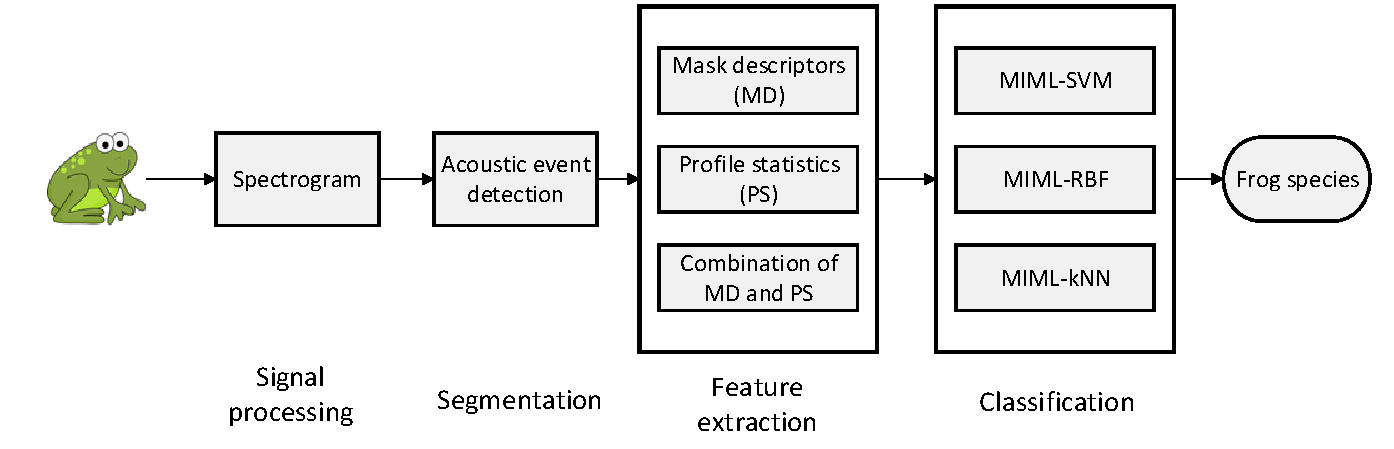
\includegraphics[width=\textwidth]{image/Ch6/flowchart.pdf}
\caption{Flowchart of a frog call classification system using MIML learning}
\label{fig:flowchart}
\end{figure}


\subsection{Materials}
\label{chap5:Materials}

All recordings were obtained from three sites in Queensland, Australia: \textit{Kiyomi dam}, \textit{Stony creek dam} and  \textit{BG creek dam}.
A battery-powered acoustic sensor (stored in a weather proof metal box) with an external microphone is used for the data collection. Collected recordings were stored on 16 GB SD cards in 64 kbps MP3 mono format. 
The recordings were collected from February, 2014 to April, 2014, because it is the breeding season in Queensland when male frogs make calls to attract females for the purpose of reproducing. Each recording starts around sunset, finishes around sunrise every day and has a duration of 12 hours. To evaluate our proposed MIML classification framework, a representative sample of 342 10-second recordings was prepared. The prepared recordings were manually labelled by an ecologist with eight frog species. Some recordings contains bird calls, insect calls, and numerous sounds, but all those sounds are regarded as the background noise. Each recording includes between one and six frog species. Following the prior work of \citep{briggs2012acoustic}, we assume that recordings without frog vocalisations can be filtered out during the segmentation process. Acoustic parameters of eight frog species averaged over three randomly selected syllables are shown in Table~\ref{tab:JCU} of Chapter~\ref{cha:cha5WaveletFeature}. Here, the acoustic parameters are used as the prior knowledge for event filtering. 



%\begin{table}[htb!]
%\centering
%\caption[Acoustic parameters]{Dominant frequency ($F_{0}$) and syllable duration ($T_{s}$) of eight frog species averaged for ten randomly selected syllables.}
%\label{tab:Ch7_parameters}
%\resizebox{0.8\textwidth}{!}{
%\begin{tabular}{llcc}
%\hline\hline
%\textbf{Frog species}       & \textbf{Code} & \multicolumn{1}{l}{\textbf{Dominant frequency (Hz)}} & \textbf{Syllable duration(ms)} \\ \hline
%\textit{Canetoad}                    & CAD           & 560                                                          &       NA                     \\ 
%\textit{Cyclorana novaehollandiae}   & CNE           & 610                                                          &       400                     \\ 
%\textit{Limnodynastes terraereginae} & LTE           & 610                                                          &          100                  \\ 
%\textit{Litoria fallax}              & LFX           & 4000                                                        &         280                       \\
%\textit{Litoria nasuta}              & LNA           & 2800                                                         &       160                      \\ 
%\textit{Litoria rothii}             & LRI           & 1800                                                         &        500                    \\ 
%\textit{Litoria rubella}             & LRA           & 2300                                                         &       580                     \\ 
%\textit{Uperolela mimula}            & UMA           & 2400                                                         &       120                     \\ \hline\hline
%\end{tabular}
%}
%\end{table}


%% Canetoad (CAD) 
%%($F_{0}$=560 Hz), Cyclorana novaehollandiae (CNE) ($F_{0}$=610 Hz), Limnodynastes terraereginae (LTE) ($F_{0}$=610 Hz), Litoria fallax (LFX) ($F_{0}$=4000 Hz), Litoria nasuta (LNA) ($F_{0}$=2800 Hz), Litoria rothii (LRI) ($F_{0}$=1800 Hz), Litoria rubella (LRA) ($F_{0}$=2300 Hz), and Uperolela mimula (UMA) ($F_{0}$=2400 Hz). Here, $F_{0}$ is the averaged dominant frequency for each frog species. 



\subsection{Signal processing}
Each recording was re-sampled at 16 kHz for generating a spectrogram using STFT. Specifically, each recording was divided into frames of 512 samples with 50\% frame overlap.
A fast Fourier transform was performed on each frame with a Hamming window, which yielded amplitude values for 256 frequency bins, each spanning 31.25 Hz. The final decibel values (S) were calculated as 
\begin{equation}
S_{tf} = 20*log_{10}(A_{tf})
\end{equation}
where $A$ denotes the amplitude value, $t=0,...,T-1$ and $f=0,...,F-1$ represent time and frequency index, $T$ and $F$ are 256 frequency bins and 625 frames, respectively. 

\subsection{Acoustic event detection for syllable segmentation}
\label{Ch5:AEDmethod}

The aim of AED is to detect a specified acoustic event in audio data. In this chapter, we use AED for frog syllable segmentation. Since all recordings are collected from the field, there are many simultaneously vocalising frog species. Traditional methods for frog syllable segmentation are based on temporal information \citep{somervuo2004classification,huang2009frog}, which cannot address those environmenal recordings. Here, we modified the AED method developed by  \cite{towsey2012toolbox} for syllable segmentation. The detail of our AED method is described as follows.
\\
\textbf{Step 1:} Wiener filtering 
\noindent
\\
A 2-Dimensional Wiener filter is applied to the spectrogram image. A $5\times5$ pixel window is found to offer a satisfactory compromise between removal of background graininess and blurring of acoustic events. Wiener filtering aims to reduce the number of very small randomly distributed acoustic events appearing in the final output.
\\
\textbf{Step 2:} Spectral subtraction
\noindent 
\\
Wiener filtering can successfully remove the graininess, but some noises, such as wind, insect, motor engine that cover the whole recording, cannot be addressed. Here, spectral subtraction is used to deal with those noises (see Algorithm 2). 


\begin{algorithm}
\DontPrintSemicolon
\KwData{$\hat{S_{tf}}$, spectrogram after Wiener filtering.}
\KwResult{$\hat{S^{'}_{tf}}=\hat{S_{tf}}$, noise reduced spectrogram.}

\Begin{
%$V \longleftarrow U$\;
%$S \longleftarrow \emptyset$\;
\textbf{Construct} an array of the modal noise values for all frequency bins;

\For{$f\in F$}{
\textbf{1}. calculate the histogram of the intensity value over each frequency bin 

\textbf{2}. smooth the histogram array with a moving average window of size 7

\textbf{3}. regard the modal noise intensity at the position of maximal bin in the left-side of the histogram
}


\textbf{Smooth} the array with a moving average filter with window of size 5;

\For{$f\in F$}{
\textbf{1}. subtract the modal noise intensity

\textbf{2}. truncated negative decibel values to zero
}
}  
\caption{Spectral Subtraction\label{IR}}

\end{algorithm}

\noindent \textbf{Step 3:} Adaptive thresholding
\\
\noindent After noise reduction, the next step is to convert a noise reduced spectrogram $\hat{S^{'}_{tf}}$ into the binary spectrogram $S^{b}_{tf}$ for the event detection. Here, an adaptive thresholding method named \textit{Otsu thresholding} \citep{otsu1975threshold} is employed to find an optimal threshold.

\begin{equation}
\phi_{b}^{2}(k)=w_{1}(k)w_{2}(k)[\mu_{1}(k)-\mu_{2}(k)]^{2}
\end{equation}
\noindent where $w_{1}(k)=\sum_{0}^{k}p(j)$ is calculated from the histogram as $k$, $p(j)=n(j)/N$ are the values of the normalised gray level histogram, $n(j)$ is the number of values in level $j$, $N$ is the total number of values over the whole spectrogram image, $\mu_{1}(k)=[\sum_{0}^{k}p(j)x(j)]/w_{1}$, $x(j)$ is the value at the center of the $j$-th histogram bin. Then, the threshold, $T_{0}$, is calculated as

\begin{equation}
T_{0}= (\phi_{b1}^{2}(k) + \phi_{b2}^{2}(k)) / 2
\end{equation}


\noindent \textbf{Step 4:} Events filtering using dominant frequency and event area \\
Since not all detected events correspond to frog vocalisations, those events that are not from the listed frog species in Table~\ref{tab:JCU} of Chapter~\ref{chap5:Materials}, dominant frequency ($F_{0}$) and area of the event ($Ar$) are used for filtering.


\noindent \textbf{Step 5:} Region growing
\\
A region growing algorithm is to obtain the contour of each segmented acoustic event \citep{mallawaarachchi2008spectrogram}. To get the accurate boundary of each acoustic event and improve the discrimination of extracted features, a 2-dimensional region growing algorithm is used to obtain the accurate event shape for each segmented event. First, the point with the maximal intensity value within the event area is selected as the seed. Then, the neighbourhood pixels of the seed(s) above the threshold are located and assigned to the output image, and new added pixels are used as seeds for further processing. Finally, when all the pixels that satisfy the criteria are added to the output image, the recursive algorithm will stop and get the final results (Figure~\ref{fig:Ch6_AED}). Here, the threshold value is empirically set as 5 dB.


\begin{algorithm}
\DontPrintSemicolon
\KwData{ $S^{b}_{tf}$, spectrogram; $t_{s}(n)$, $t_{e}(n)$, $f_{l}(n)$, $f_{h}(n)$, location of each acoustic event $n$; $F_{0}(i)$, dominant frequency of frog species $i$.}
\KwResult{ $\tilde{S_{tf}}$, spectrogram after events filtering.}

\Begin{
%\textbf{Step 1:} separate large acoustic events
%\\
\textbf{Calculate} the area of each acoustic event $n$.
$Area(n)=(t_{e}(n)-t_{s}(n))*(f_{h}(n)-f_{l}(n))$

\For{$n \in N_{e1}$}{
\If{$Ar(n) \geq Ar_{l}$}{
split event $n$ into small events
}
} 
where $Ar_{l}$ is set as 2000 pixels.\\
%\textbf{Step 2:} dominant frequency 
\textbf{Filter} events using dominant frequency
$f_{d}(n)= \sum_{t=t_{s}(n)}^{t_{e}(n)} F(t) / t_{e}(n)-t_{s}(n)$ \\
where $F(t)$ is the peak frequency of each frame within the event area


\For{$n \in N_{e2}$}{
\For{$i \in I$}{
\If{$f_{d}(n) \geq F_{0}(i)+\theta$; $f_{d}(n) \leq F_{0}(i)-\theta$}{
	$f_{d}(n) =0$;
}
}}
where $\theta$ is frequency range and set as 300 Hz.

\textbf{Remove} small acoustic events except frequency band between $\theta_{l}$ and $\theta_{h}$
\\
\For{$n \in N_{e2}$}{
\If{$Ar(n) \leq Ar_{s}$}{
remove event $n$
}
} 
where $Ar_{s}$ is set as 200 pixels, $\theta_{l}$ and $\theta_{h}$ are set as 300 Hz and 800 Hz, respectively. Because the area of \textit{LTE} is smaller than $Ar_{s}$.
}
\caption{Event filtering based on dominant frequency and event area}
\end{algorithm}






\begin{figure}[htb!]
\centering

        \begin{subfigure}[b]{0.45\textwidth}
                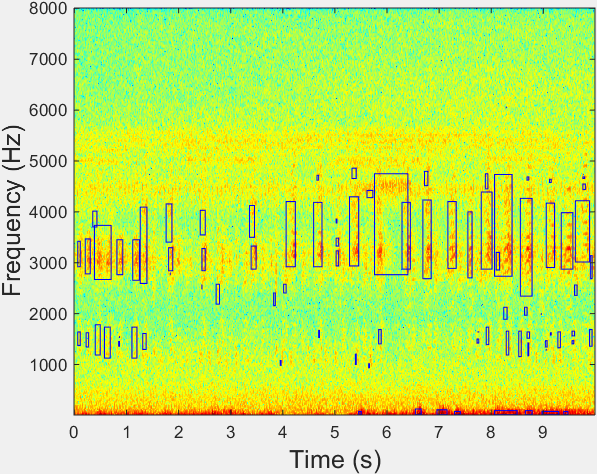
\includegraphics[width=\textwidth, height =0.8 \textwidth]{image/Ch6/AEoriginal.png}
                %\caption{ }
        \end{subfigure}
       ~
              \begin{subfigure}[b]{0.45\textwidth}
                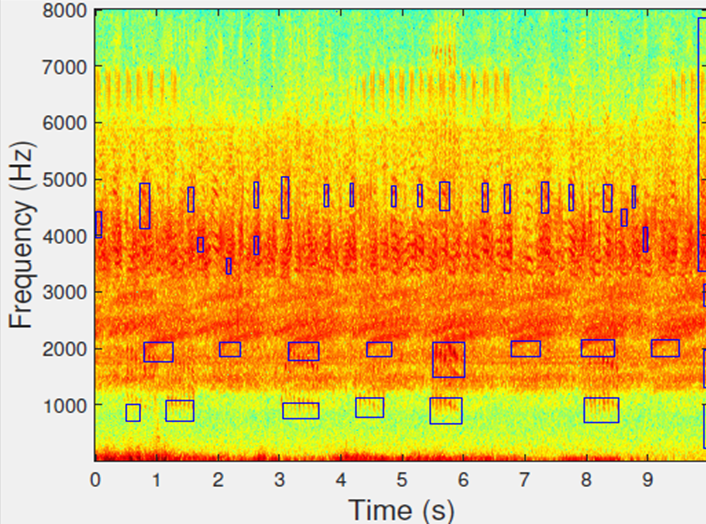
\includegraphics[width=\textwidth,height = 0.8 \textwidth]{image/Ch6/AEfinal.png}                
        \end{subfigure}     
\caption[Acoustic event detection results]{Acoustic event detection results before (Left) and after (Right) event filtering based on dominant frequency. Here, blue rectangle denotes the time and frequency boundary of each detected event}
        \label{fig:feature}
\end{figure}

%\begin{figure}[htb!]
%\centering
%        \begin{subfigure}[b]{0.45\textwidth}
%                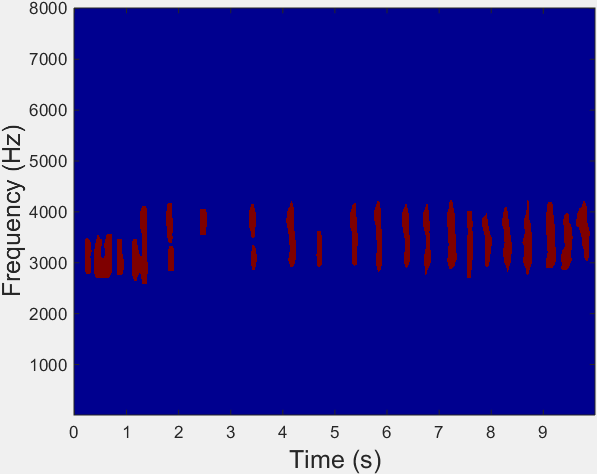
\includegraphics[width=\textwidth]{image/Ch6/binary.png}
%                %\caption{ }
%        \end{subfigure}
%       ~
%              \begin{subfigure}[b]{0.45\textwidth}
%                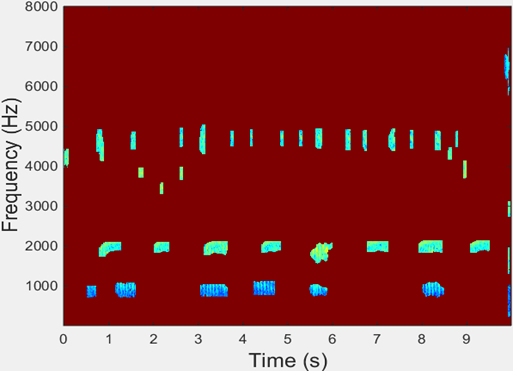
\includegraphics[width=\textwidth]{image/Ch6/segmentEvents.png}                
%        \end{subfigure}       
%\caption[Acoustic event detection results after region growing]{Acoustic event detection results after region growing. Left: binary segmentation results; Right: segmented frog syllables.}
%        \label{fig:Ch6_AED}
%\end{figure}

\begin{figure}[htb!]
\centering
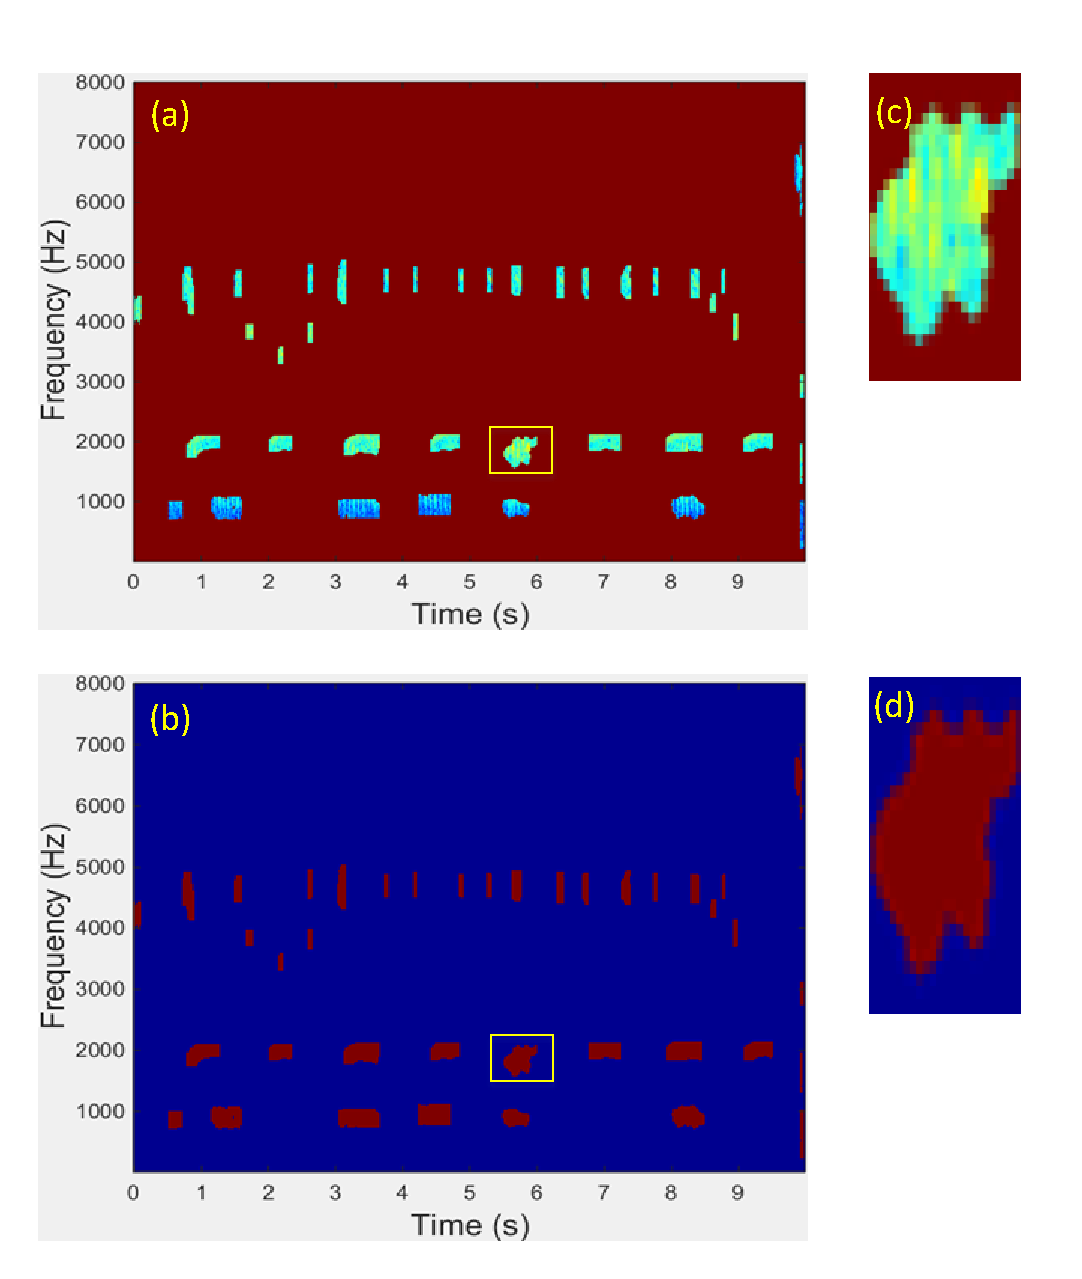
\includegraphics[width=0.75\textwidth, height = 0.9\textwidth]{image/Ch6/contentShape.pdf}
\caption[Acoustic event detection results after region growing]{Acoustic event detection results after region growing. (a) binary segmentation results, (b) segmented frog syllables. (c) The masked and cropped spectrogram corresponding to the highlighted segment. (d) A cropped mask of the highlighted segment}
\label{fig:Ch6_AED}
\end{figure}






\subsection{Feature extraction}
To compute features for each segment, the spectrogram and mask will be first cropped to contain just one segment. Figures~\ref{fig:Ch6_AED}(c) and \ref{fig:Ch6_AED}(d) show a cropped image of the spectrogram and mask based on the highlighted segment.
To describe the segment features, notation will be used as follows:
Let $M_{t,f}$ be the cropped, binary mask for a segment, and let $\bar{S}_{t,f}$ be the cropped, original spectrogram. Note that $t$ ranges from 1 to the duration of the segment in frames, $T$.



Two feature sets are calculated to describe each segment (syllable): mask descriptors and profile statistics \citep{briggs2012acoustic}. Here, we exclude \textit{histogram of orientation (HOG)} from our feature set for its poor classification performance in previous studies \citep{briggs2012acoustic, ruizmultiple2015}. 

\noindent \textbf{Mask descriptors}
\\
Mask descriptors for a segment are based on only the mask, and describe the shape of the segment. The features are
\\
\noindent (1) Min-frequency = min \{f: $M_{t,f}$ = 1 \} 
\\
\noindent (2) Max-frequency = max \{f: $M_{t,f}$ = 1 \}
\\
\noindent (3) Bandwidth = max-frequency - min-frequency
\\
\noindent (4) Duration = $T$
\\
\noindent (5) Area = $\sum_{tf}M_{tf}$
\\
\noindent (6) Perimeter = $\frac{1}{2} \times $ ( $\#$ of pixels in $M_{t,f}$ such that at least one pixel in the surrounding 3 $\times$ 3 box is 1 and at least one pixel is 0)
\\
\noindent (7) Non-compactness = $perimeter^{2}/area$
\\
\noindent (8) Rectangularity = $area/(bandwidth \times duration)$



\noindent \textbf{Profile statistics}
\\
Profile statistics are calculated based on statistical properties of the time and frequency profiles of each segment. 
To compute the time or frequency file, the columns or rows of the spectrogram are first summed.
The time profile is $p_{t}(t) = \sum_{f}\hat{S}_{t,f}$ and the frequency profile is $p_{f}(f) = \sum_{t}\hat{S}_{t,f}$. The profiles are normalised to sum to 1, and are further interpreted as probability mass functions. The normalised profile densities are $\hat{p}_{t}$ and $\hat{p}_{f}$.
Two features measure the uniformity of the densities according the Gini index are
\\
(1) Freq-gini = 1 - $\sum_{f}\hat{p}_{f}(f)^{2}$
\\
(2) Time-gini = 1 - $\sum_{t}\hat{p}_{t}(t)^{2}$

Several more features are calculated by computing the $k$-th moments of the time and frequency profiles. Since different segments have different durations, all those features are calculated in a re-scaled coordinate system, where time is from 0 to 1 over the duration of the segment, and frequency is from 0 to 1.
\\
(3) Freq-mean = $\mu_{f}$ = $\sum_{f=1}^{f_{max}}\hat{p}_{f}(f)(f/f_{max})$
\\
(4) Freq-variance = $\sum_{f=1}^{f_{max}}\hat{p}_{f}(f)(\mu_{f}-f/f_{max})^{2}$
\\
(5) Freq-skewness = $\sum_{f=1}^{f_{max}}\hat{p}_{f}(f)(\mu_{f}-f/f_{max})^{3}$
\\
(6) Freq-kurtosis = $\sum_{f=1}^{f_{max}}\hat{p}_{f}(f)(\mu_{f}-f/f_{max})^{4}$
\\
(7) Time-mean =  $\mu_{t}$ = $\sum_{t=1}^{t_{max}}\hat{p}_{t}(t)t/T)$
\\
(8) Time-variance = $\mu_{t}$ = $\sum_{t=1}^{t_{max}}\hat{p}_{t}(t)t/T)^{2}$
\\
(9) Time-skewness = $\mu_{t}$ = $\sum_{t=1}^{t_{max}}\hat{p}_{t}(t)t/T)^{3}$
\\
(10) Time-kurtosis = $\mu_{t}$ = $\sum_{t=1}^{t_{max}}\hat{p}_{t}(t)t/T)^{4}$
\\
Also, the maxima of the time and frequency profiles are calculated
\\
(11) Freq-max = $(argmax \hat{p}_{f}(f)) / f_{max}$
\\
(12) Time-max = $(\hat{p}_{f}(t)) / T$

The mean and standard deviation of the spectrogram within the masked region are further calculated.
\\
(13) Mask-mean = $\mu_{tf}$ = $(1/area) \sum_{tf}\hat{S}_{tf}$
\\
(14) Mask-stddev = $\sqrt{(1/area) \sum_{tf}(\mu_{tf}-\hat{S}_{tf})^{2}}$


Besides mask descriptors (MD) and profile statistics (PS), a third feature set is constructed with all features.

All of the features used to describe the segment are concatenated to form a single feature vector, but the values differ widely from each other. This property will affect the classification performance especially the distance-based classifier, where more weight will be placed on features with larger magnitudes. To prevent this bias, all those features are rescaled to [0,1] independently.



\subsection{Multiple-instance multiple-label classifiers}
After feature extraction, three MIML algorithms are evaluated for the classification of multiple simultaneous vocalising frog species: MIML-SVM, MIML-RBF, and MIML-kNN. 
These algorithms reduce the MIML problem to single-instance multiple-label problem by associating each bag (10-second recording) with a bag-level feature, which aggregates information from the instances in the bag  \citep{briggs2012acoustic}. Each algorithm constructs different bag-level features, but all use some form of bag-level distance measure. Here, the maximal and average Hausdorff distances between two syllables are used by MIML-SVM and MIML-RBF, respectively. For MIML-kNN, the nearest neighbour is used to assign bag-level features. 


\section{Experiment results}

\subsection{Parameter tuning}
There are three modules, the parameters of which need to be discussed: signal processing, acoustic event detection, and classification. For signal processing, the window size and overlap are 512 samples and 50\%, respectively. During the process of acoustic event detection, four thresholds for event filtering need to be determined, which are small and large area threshold, and frequency boundary for events filtering. All those thresholds were determined empirically by applying various combinations of thresholds to the constructed validation dataset. For MIML-SVM classifiers, the parameters used are ($C,\gamma,r$) and set as (0.1, 0.6, 0.2) experimentally. For MIML-RBF, the parameters are ($ r, \mu$) and set as (0.1,0.6). For MIML-kNN, the number of references (k) and citers ($k^{'}$) are 10 and 20, respectively. Note that the dataset used for parameter setting is excluded from the testing dataset.
 
%Five measures including Hamming loss, rank loss, one-error, coverage, and micro-AUC are used to characterize the accuracy of each algorithm \cite{zhou2008miml, dimou2009empirical}. The definition of each measure can be found in \cite{briggs2012acoustic}


\subsection{Classification}

\label{ch6:eveluationMetric}
In this chapter, all the algorithms are programmed in Matlab 2014b. Each MIML algorithm is evaluated with five-fold cross-validation on the collection of 342 species-labelled recordings. 
Five evaluation metrics are used for comparing the performance with the combination of three feature sets and three MIML algorithms: Hamming loss, Rank loss, One error, coverage, and  average precision \citep{Madjarov20123084, zhou2008miml}. The value range of all five evaluation rules is between 0 to 1. The definition of each evaluation rule is described as follows:
\\
\textbf{(1)} Hamming loss is defined as the fraction of labels that are incorrectly predicted for an instance and the normalised Hamming loss which is normalised over instances is reported. This metric is defined as
\begin{equation}
hammingLoss = \frac{1}{N}\sum_{i=1}^{N}\frac{1}{Q}|h(x_{i})\Delta y_{i})|
\end{equation}
where $\Delta$ denotes the symmetric difference between two instances, $N$ is the number of instances and $Q$ is the total number of possible labels. $y_{i}$ denotes the ground truth of instance $x_{i}$, and $h(x_{i})$ denotes the predictions for the same instance. 
\\
\textbf{(2)} Ranking loss evaluates the average fraction of label pairs that are reversely ordered for the particular instance given by
\begin{equation}
rankingLoss = \frac{1}{N}\sum_{i=1}^{N}\frac{|D_{i}|}{|y_{i}||\bar{y_{i}}|}
\end{equation}
where $D_{i}={(\lambda_{m},\lambda_{n})| f(x_{i}, \lambda_{m}) \leq f(x_{i}, \lambda_{n}), (\lambda_{m}, \lambda_{n}) \in y_{i} \times \hat{y_{i}}}$,
while $\bar{y}$ denotes the complementary set of $y$ in $L$, and $L={\lambda_{1}, \lambda_{2}, \lambda_{3},..., \lambda_{Q}}$, $\lambda$ represents the label.
\\
\textbf{(3)} One error evaluates how many times the top-ranked label is
not in the set of relevant labels of the instance. This evaluation metric is defined as

\begin{equation}
oneError = \frac{1}{N}\sum_{i=1}^{N}[[argmax_{\lambda \in y} f(x_{i},\lambda)] \not \in y_{i} ]
\end{equation}
\\
\textbf{(4)} 
Coverage evaluates how far, on average, we need to go down
the list of ranked labels in order to cover all the relevant labels of the example. The definition of this metric is shown as
\begin{equation}
coverage(f)= \frac{1}{N}\sum_{i=1}^{N} max {rank_{f}(x_{i}, \lambda)-1}
\end{equation}
where $rank_{f}(x_{i}, \lambda)$ maps the outputs of $f(x_{i}, \lambda)$ for any
$\lambda \in L$ to ${\lambda_{1},\lambda_{2},...,\lambda_{Q}}$, so that 
$f(x_{i}, \lambda_{m}) \leq f(x_{i}, \lambda_{n})$ implies 
$rank_{f}(x_{i}, \lambda_{m}) \leq rank_{f}(x_{i}, \lambda_{n})$ 
\\
\textbf{(5)} 
Average precision is the average fraction of labels that are ranked higher than an actual label belonging to an instance. 
\begin{equation}
avgPrecision = \frac{1}{N}\sum_{i=1}^{N}\frac{h(x_{i}) \cap y_{i}}{|y_{i}|}
\end{equation}

The values for hamming loss, rank loss, one-error, coverage, and average precision range from 0 to 1. For hamming loss, rank loss, one-error, and coverage, 0 denotes the perfect result, and 1 means the wrong prediction of all labels over every instance, whereas for average precision, the values have the completely opposite meanings. 



\subsection{Results}

The classification results are shown in Figure~\ref{fig:classificationResults}. To obtain a base line for hamming loss, a non-informative classifier is always considered to predict the empty set. The baseline of hamming loss is thus calculate as $m/c$, where $c$ is the number of frog species to be classified, $m$ is calculated as $(1/n)\sum_{i=1}^{n}|Y_{i}|$. Here, the value of baseline of hamming loss is 0.3220. It can be found that the hamming loss for MIML-RBF with AF is 2.70 times better than the non-informative classifier. With a rank loss of 0.0831, MIML-RBF with AF is 6.01 times better than the non-informative classifier. A one error of 0.1438 means that if we only predict the highest scoring species in each recording, it will truly be present 85.62\% of the time. 
The $positive/negative$ is defined as $1-hammingLoss$ and it is 88.08\% for MIML-RBF with AF. Compared to MIML-kNN and MIML-SVM,  MIML-RBF is found to achieve the best classification performance. For those three feature sets, the hamming loss for AF is always better than PS and MD. 



\begin{figure}[htb!]
\centering

        \begin{subfigure}[b]{0.45\textwidth}
                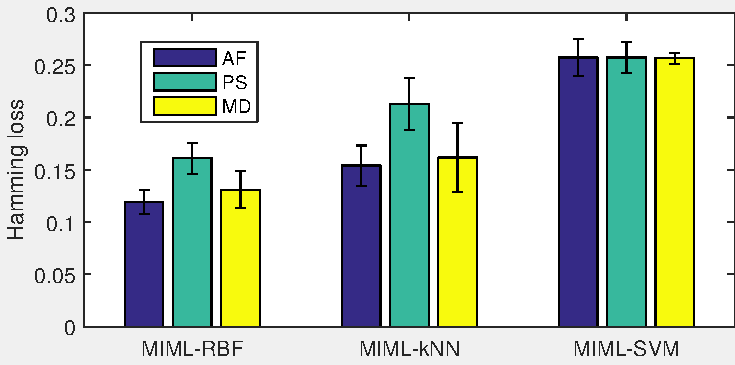
\includegraphics[width=\textwidth]{image/Ch6/hammingLoss.pdf}
                \caption{Hamming loss}
        \end{subfigure}
       ~
              \begin{subfigure}[b]{0.45\textwidth}
                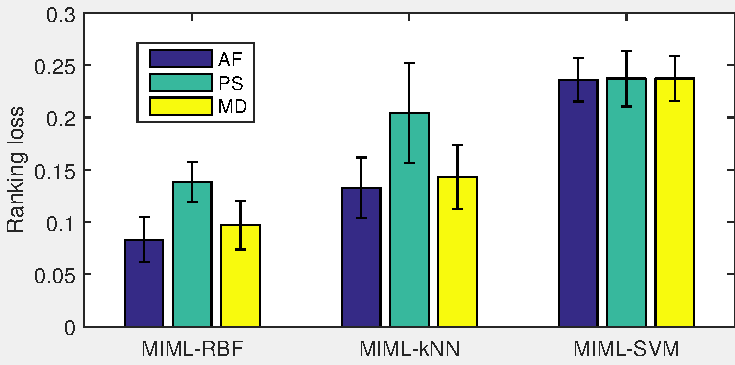
\includegraphics[width=\textwidth]{image/Ch6/rankingLoss.pdf}
                                \caption{Rank loss}               
        \end{subfigure}  
     \\
              \begin{subfigure}[b]{0.45\textwidth}
                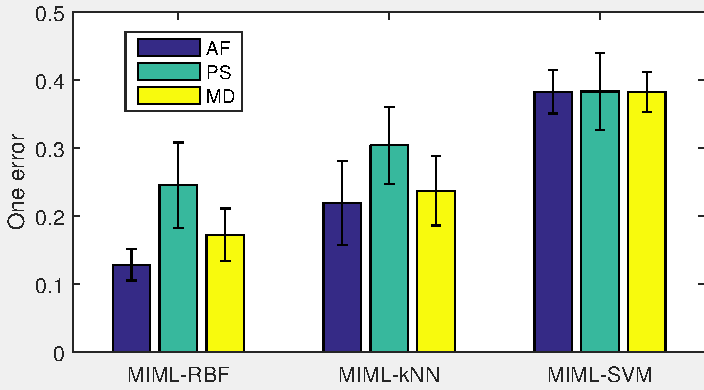
\includegraphics[width=\textwidth]{image/Ch6/oneError.pdf} 
                \caption{One error}               
        \end{subfigure}  
~
              \begin{subfigure}[b]{0.45\textwidth}
                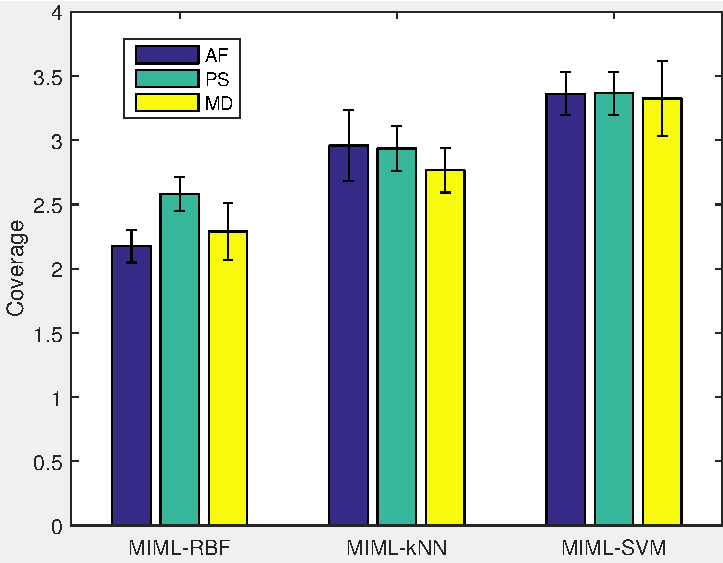
\includegraphics[width=\textwidth]{image/Ch6/coverage.pdf} 
                \caption{Coverage}                
        \end{subfigure}          
   \\
              \begin{subfigure}[b]{0.45\textwidth}
                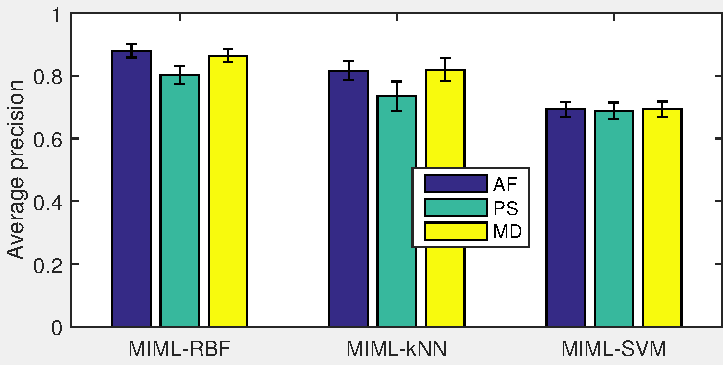
\includegraphics[width=\textwidth]{image/Ch6/avgPrecision.pdf}  
                     \caption{Average precision}         
        \end{subfigure}      
\caption[MIML classification results]{Evaluation metrics for MIML classifiers with three different feature sets}
        \label{fig:classificationResults}
\end{figure}

To give a concrete view of predictions, the results of five randomly selected recordings using MIML-RBF are shown in Table~\ref{tab:prediction}. From the table, we can see that recordings of No.4 are accurately predicted. Recordings of No.1, No.2, and No.3 are partially accurate. Recording of No.5 is wrongly predicted.

\begin{table}[htb!]
\centering
\caption{Example predictions with MIML-RBF using AF}
\label{tab:prediction}
\begin{tabular}{lll}
\hline\hline
{\bf No.} &{\bf Ground truth} & {\bf Predicted labels} \\ \hline
1&LNA, UMA                & LNA,LRA                    \\ 
2&UMA      &     LNA, UMA      \\ 
3& UMA           & LNA, UMA               \\ 
4&LNA, UMA      & LNA, UMA     \\ 
5&UMA      & LNA            \\ \hline\hline
\end{tabular}
\end{table}


In this chapter, all the features are directly calculate based on AED results.
It is obviously that different AED results will lead to different classification results. 
A comparison of three AED methods is shown in Table~\ref{Ch6:AEDCompare}, where features and classifier used are the same. The results show that our proposed AED method can achieve the best classification performance.


%\begin{table}[htb!]
%\centering
%\caption{Effects of AED for the MIML classification results. Here, $\downarrow$ indicates that smaller values imply higher accuracy, while ‘$\uparrow$’ has the completely opposite meanings.}
%\label{Ch6:AEDCompare}
%\begin{tabular}{llllll}
%\hline\hline
%AED     & Feature & Classifier & Hamming loss $\downarrow$ & Coverage $\downarrow$     & Average Precision  $\uparrow$\\ \hline
%Ours    &       &    & 0.1136 $\pm$ 0.0145 & 2.4873 $\pm$ 0.2460 & 0.8739 $\pm$ 0.0272     \\ 
%Michael & AF      & MIML-RBF   & 0.1231 $\pm$ 0.0116 & 2.6820 $\pm$ 0.1622 & 0.8313 $\pm$ 0.0250     \\ 
%Fodor   &       &   & 0.1657 $\pm$ 0.0053 & 2.9563 $\pm$ 0.2137 & 0.8074 $\pm$ 0.0122     \\ \hline\hline
%\end{tabular}
%\end{table}


\begin{table}[htb!]
\centering
\caption[Effects of AED on the MIML classification results]{Effects of AED for the MIML classification results. Here, $\downarrow$ indicates that smaller values imply higher accuracy, while ‘$\uparrow$’ has the completely opposite meanings}
\label{Ch6:AEDCompare}
\begin{tabular}{llllll}
\hline\hline
AED     & Feature & Classifier & Hamming loss $\downarrow$ & Coverage $\downarrow$     & Average Precision  $\uparrow$\\ \hline
Ours    & AF      & MIML-RBF   & \textbf{0.1192 $\pm$ 0.0112} & \textbf{2.1614 $\pm$ 0.1516} & \textbf{0.8793 $\pm$ 0.0213}     \\ 
Michael & AF      & MIML-RBF   & 0.1275 $\pm$ 0.0090 & 2.2690 $\pm$ 0.1177 & 0.8529 $\pm$ 0.0217     \\ 
Fodor   & AF      & MIML-RBF   & 0.1777 $\pm$ 0.0131 & 2.5471 $\pm$ 0.1339 & 0.8265 $\pm$ 0.0287     \\ \hline\hline
\end{tabular}
\end{table}




\section{Discussion}
Since most recordings in this chapter contain multiple simultaneously vocalising frog species, the traditional SISL classification framework is no longer suitable. A novel framework for the classification of multiple simultaneous vocalising frog species in field recordings is proposed, which is adopted from \citep{briggs2012acoustic}, a study on birds. Different from their work, this research designs a new AED method for frog syllable segmentation rather than using a supervised learning algorithm. It is because that there are few annotated frog recordings. Since all the features in this study are calculated from the segmented syllables, the accuracy of the segmentation results directly affects the final classification performance. Compared to other two AED methods, extracting features based on our AED results can achieve better classification performance (Table~\ref{Ch6:AEDCompare}).

We also investigate SISL classification results using a small dataset. Total 176 10-second recordings are annotated using eight frog species. On the average, each 10-second recording has 19.5 frog syllables. For SISL classification, MFCCs and AWSCCs are used as the features, respectively. The window size and overlap for calculating MFCCs and AWSCCs are 128 samples and 50\%, which are selected according to Chapter~\ref{cha:cha4EnhancedFeature}. RF is used as the classifier for its best classification performance in Chapter~\ref{cha:cha4EnhancedFeature}. 
The MIML classification results are achieved using the combination of AF and MIML-RBF. The precision and recall for MIML and SISL classification are shown in Figure~\ref{fig:comparisonofSISLandMIML}. Generally, MIML can achieve better performance than SISL for all frog species except for \textit{RMA}. The high classification performance for \textit{RMA} using SISL might be that frequency structure of \textit{RMA} is much clearer than other frog species. Among all frog species, precision and recall are higher than 0.6 for MIML. Both precision and recall of \textit{LNA} and \textit{UMA} are 1, which are much higher than other frog species. The reasons for this high classification performance might be that the cepstral domain information of \textit{LNA} and \textit{UMA} can be better described by MFCCs. For SISL, \textit{LUA} and \textit{LFX} has the poorest classification performance. The reasons for poor classification accuracy of \textit{LFX} might be insufficient training instances and inappropriate features for this frog species. Compared to MFCCs, our propose AWSCCs in Chapter~\ref{cha:cha5WaveletFeature}.


\begin{figure}[htb!]
\centering
        \begin{subfigure}[b]{0.48\textwidth}
                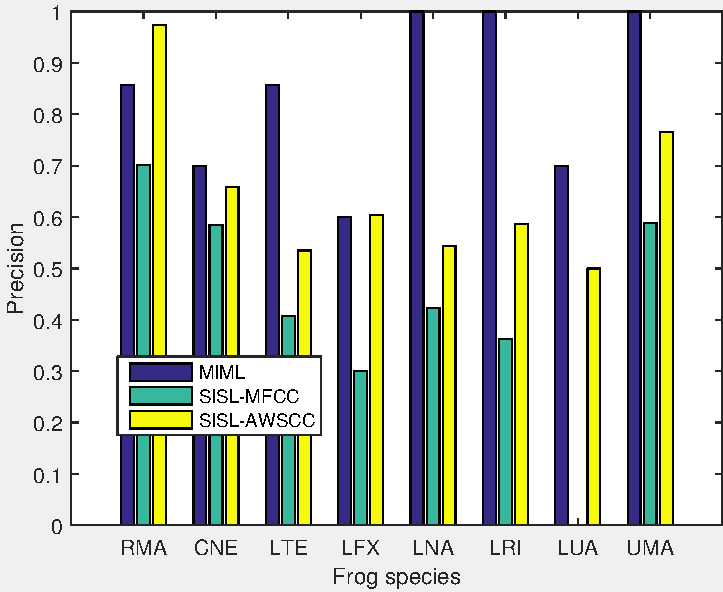
\includegraphics[width=\textwidth]{image/Ch6/Precision_MIML_SISL_2.pdf}
                %\caption{ }
        \end{subfigure}
       ~
              \begin{subfigure}[b]{0.48\textwidth}
                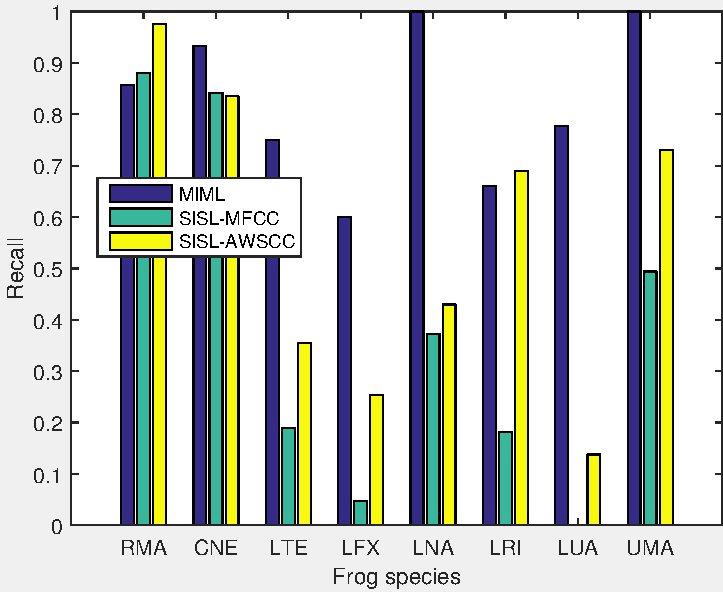
\includegraphics[width=\textwidth]{image/Ch6/Recall_MIML_SISL_2.pdf}                
        \end{subfigure}     
\caption[Comparisons between SISL and MIML]{Comparisons of precisions and recalls between SISL and MIML classification for eight frog species}
        \label{fig:comparisonofSISLandMIML}
\end{figure}



\begin{figure}[htb!] % Example image
\center{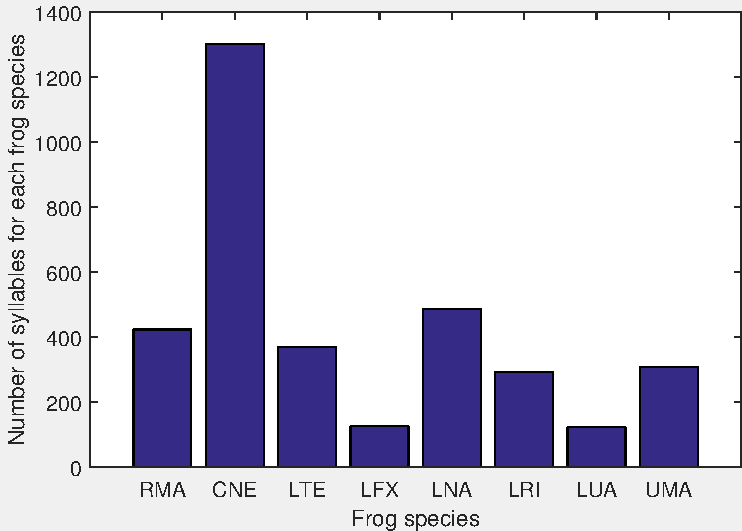
\includegraphics[width=0.6\linewidth]{image/Ch6/FrogSyllable.pdf}}
\caption[Distribution of syllable number for all frog species]{Distribution of syllable number for all frog species. The x-axis is the abbreviation of each frog species, and the corresponding scientific name can be found in Table \ref{tab:JCU}}
\label{fig:Ch6_syllable} 
\end{figure}

\section{Summary}
In this chapter, we propose a novel MIML classification framework for classifying multiple simultaneously vocalising frog species in field recordings. To the best of this author's knowledge, this is the first study that focuses on frog recordings using MIML learning. Since multiple frog species tend to call simultaneously, MIML learning is a natural fit for dealing with those recordings than SISL learning. For frog syllable segmentation, our propose AED method can achieve the best performance, which can be reflected by the classification results. Compared to SISL classification, MIML classification can achieve higher classification performance. Current classification results are found to be highly affected by the syllable segmentation results, and the use of AED cannot accurately segment all the syllables. One solution is to prepare an annotated dataset and apply supervised learning algorithms for the segmentation task. Another is to use a different classification framework, which does not need the segmentation process, and we examine this option in the next chapter.


